\documentclass[12pt]{article}

\usepackage[margin=1in]{geometry} 
\usepackage{amsmath,amsthm,amssymb}
\usepackage[spanish]{babel}
\usepackage[utf8]{inputenc}
\usepackage{tikz-cd}
\usepackage{amsmath}
\usepackage[shortlabels]{enumitem}
\usepackage{mathtools}
\usepackage{float}
\usepackage{listings}
\usepackage{xcolor}
\usepackage{url}

\graphicspath{{img/}}

\title{SWAP: Práctica 6}
\author{
        Antonio Gámiz Delgado
}

\begin{document}

\maketitle

\section{Configuar servidor NFS}

Primero creamos la máquina que va a hacer de \textit{NFS}:

\begin{figure}[H]
\center
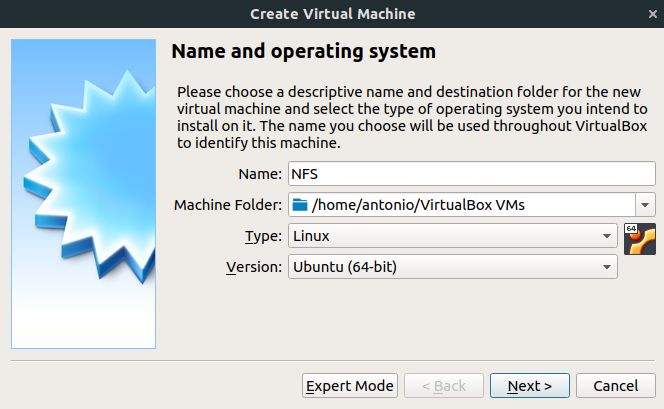
\includegraphics[scale=0.4]{1.png}
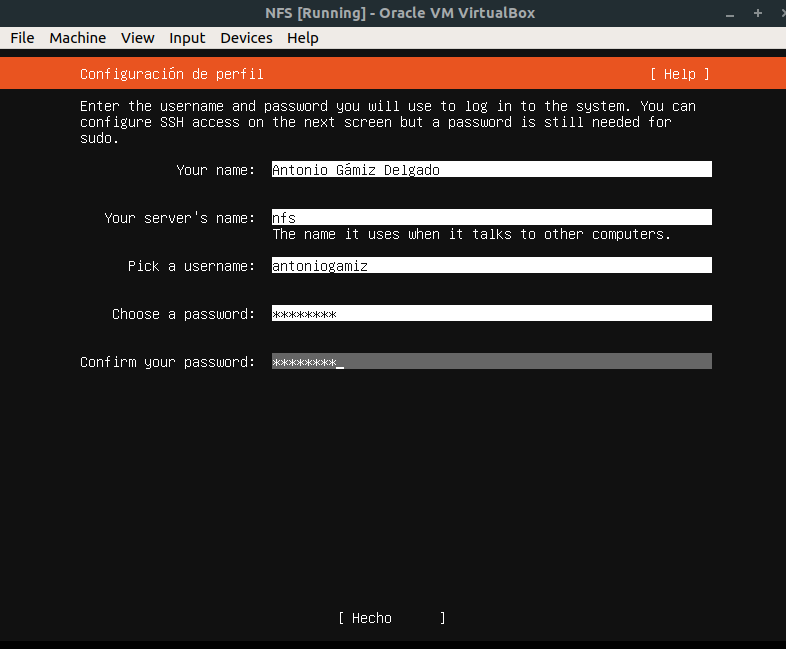
\includegraphics[scale=0.3]{2.png}
\end{figure}

Ahora añadimos el adaptador de red:

\begin{figure}[H]
\center
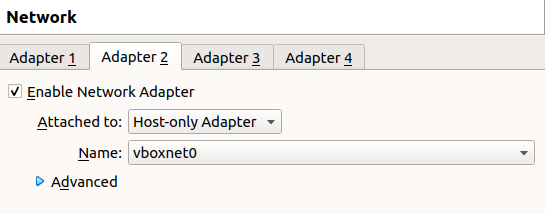
\includegraphics[scale=0.4]{3.png}
\end{figure}

Y realizamos la configuración necesaria en \textit{netapply}:

\begin{figure}[H]
\center
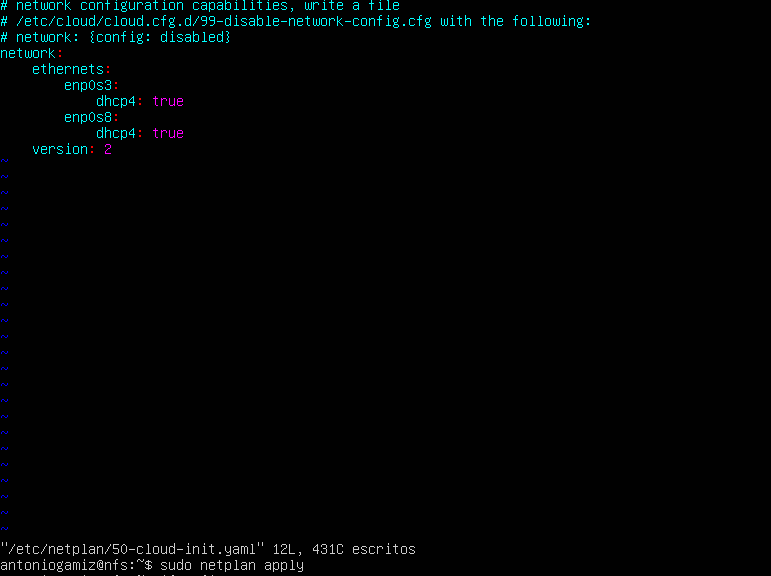
\includegraphics[scale=0.4]{4.png}
\end{figure}

Ya tenemos el host listo para usar y conectarnos mediante \textit{ssh}. Ahora instalamos las herramientas necesarias para utilizarla como servidor \textit{NFS}:

\begin{figure}[H]
\center
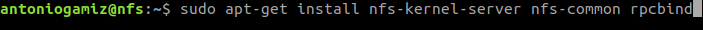
\includegraphics[scale=0.4]{6.png}
\end{figure}

Después creamos la carpeta que vamos a compartir con los clientes y cambiamos el propietario y permisos de esa carpeta:

\begin{figure}[H]
\center
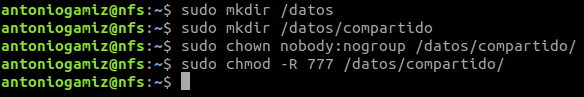
\includegraphics[scale=0.4]{7.png}
\end{figure}

Para dar permiso de acceso a las máquinas clientes, debemos añadir las IP correspondientes en el archivo de configuración:

\begin{figure}[H]
\center
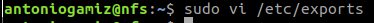
\includegraphics[scale=0.4]{9.png}
\end{figure}
\begin{figure}[H]
\center
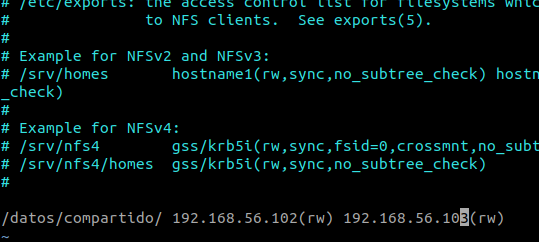
\includegraphics[scale=0.4]{8.png}
\end{figure}

Finalmente, debemos reiniciar el servicio y comprobar que está todo correcto:

\begin{figure}[H]
\center
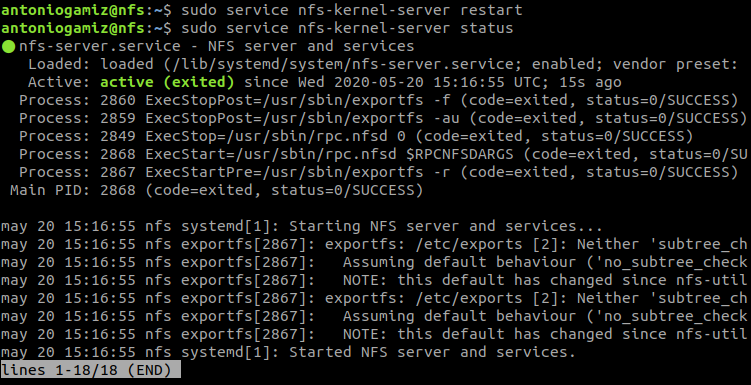
\includegraphics[scale=0.4]{10.png}
\end{figure}

\section{Configurar los clientes M1 y M2}

En los clientes debemos instalar los paquetes 
necesarios y crear el punto de montaje:

\medskip

\centerline{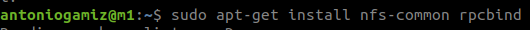
\includegraphics[scale=0.6]{11.png}}

\centerline{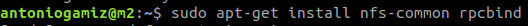
\includegraphics[scale=0.6]{12.png}}

\centerline{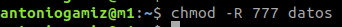
\includegraphics[scale=0.6]{13.png}}

\centerline{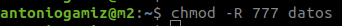
\includegraphics[scale=0.6]{14.png}}

Ahora ya podemos montar la carpeta remota (la exportada en el servidor NFS) sobre el directorio recién creado:\\

\centerline{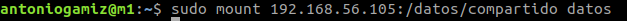
\includegraphics[scale=0.6]{15.png}}

\centerline{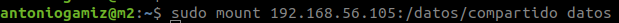
\includegraphics[scale=0.6]{16.png}}

Ahora comprobamos que todo funciona correctamente creando un archivo en M1 y viendo que se replica en M2 y en NFS:\\

\centerline{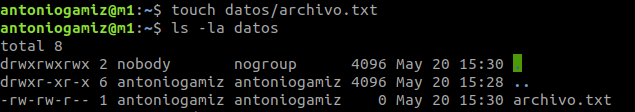
\includegraphics[scale=0.6]{17.png}}

\centerline{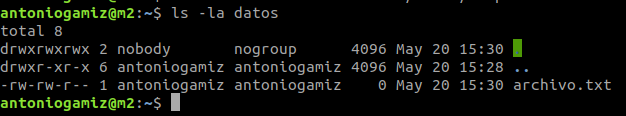
\includegraphics[scale=0.6]{18.png}}

\centerline{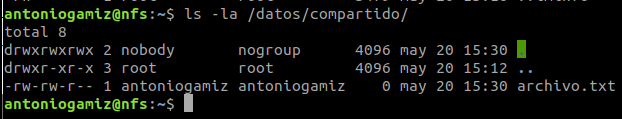
\includegraphics[scale=0.6]{19.png}}


Finalmente, para hacer la configuración permanente, debemos añadir una línea al archivo de configuración \textit{/etc/fstab} para que la carpeta compartida se monte al arrancar el sistema:\\


\centerline{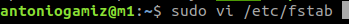
\includegraphics[scale=0.6]{20.png}}

\centerline{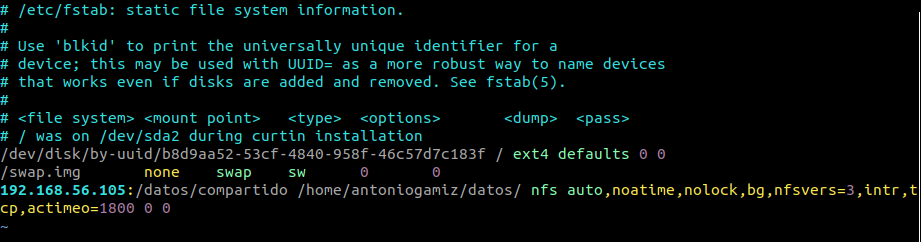
\includegraphics[scale=0.5]{21.png}}

\medskip

\centerline{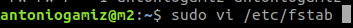
\includegraphics[scale=0.6]{22.png}}

\centerline{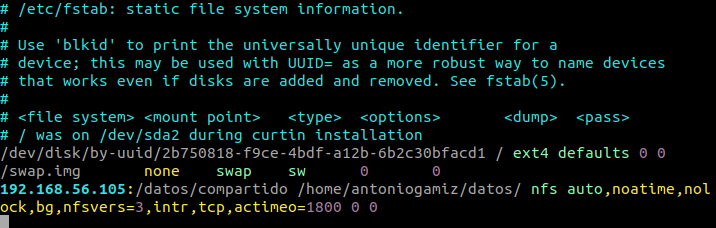
\includegraphics[scale=0.5]{23.png}}

\end{document}